\documentclass{beamer}
\usepackage[utf8]{inputenc}
\usepackage[T1]{fontenc}
\usepackage{lipsum, lmodern}
\usepackage[scaled=.95]{helvet}% helvetica as the origin of arial
\usepackage[helvet]{sfmath}    % for the mathematical enviroments
\usepackage{braket}
\usepackage{physics}
\usepackage{xcolor}
\renewcommand{\familydefault}{\sfdefault}

%% ETH beamer theme
% Options: [default]
%   itemsblack/[itemsblue]: change color of bullets etc. to black/blue in itemize style environments
%   [titlesblack]/titlesblue: change color of frame titles/subtitles to black/blue
% \usetheme[itemsblack,titlesblack]{eth}
\usetheme{eth}

%% Theme uses ETH blue color by default. Can be changed to any color using this command: 
% \setbeamercolor{structure}{fg=blue}

%% Mandatory variables
\author{Matteo Bellino}
\title{Super-radiant and Sub-radiant Cavity Scattering by Atom Arrays}
\subtitle{Z. Yan \textit{et alii}, Phys. Rev. Lett \textbf{131} (2023)}
\date{February 27, 2025}

%% Optional variables
% \supervisor{Jane Smith} % for one supervisor
% \supervisors{Carol Foote, Jane Smith} % for multiple supervisors
%\projecttype{More Advanced Topics in Quantum Optics}

\begin{document}
\frame{\maketitle}
\begin{frame}{Definition}
	\alert{\textit{Super-radiance}} refers to the situation where, due to coherent constructive interference of the light scattered by different atoms, the cavity light's intensity scales up quadratically with the number $N$ of scatterer atoms.\newline
	~\newline
	On the contrary, \alert{\textit{sub-radiance}} refers to a sub-linear scaling of the scattered light's intensity with $N$.
\end{frame}

\begin{frame}{Experimental setup}
	\begin{minipage}{\textwidth}
		\centering
		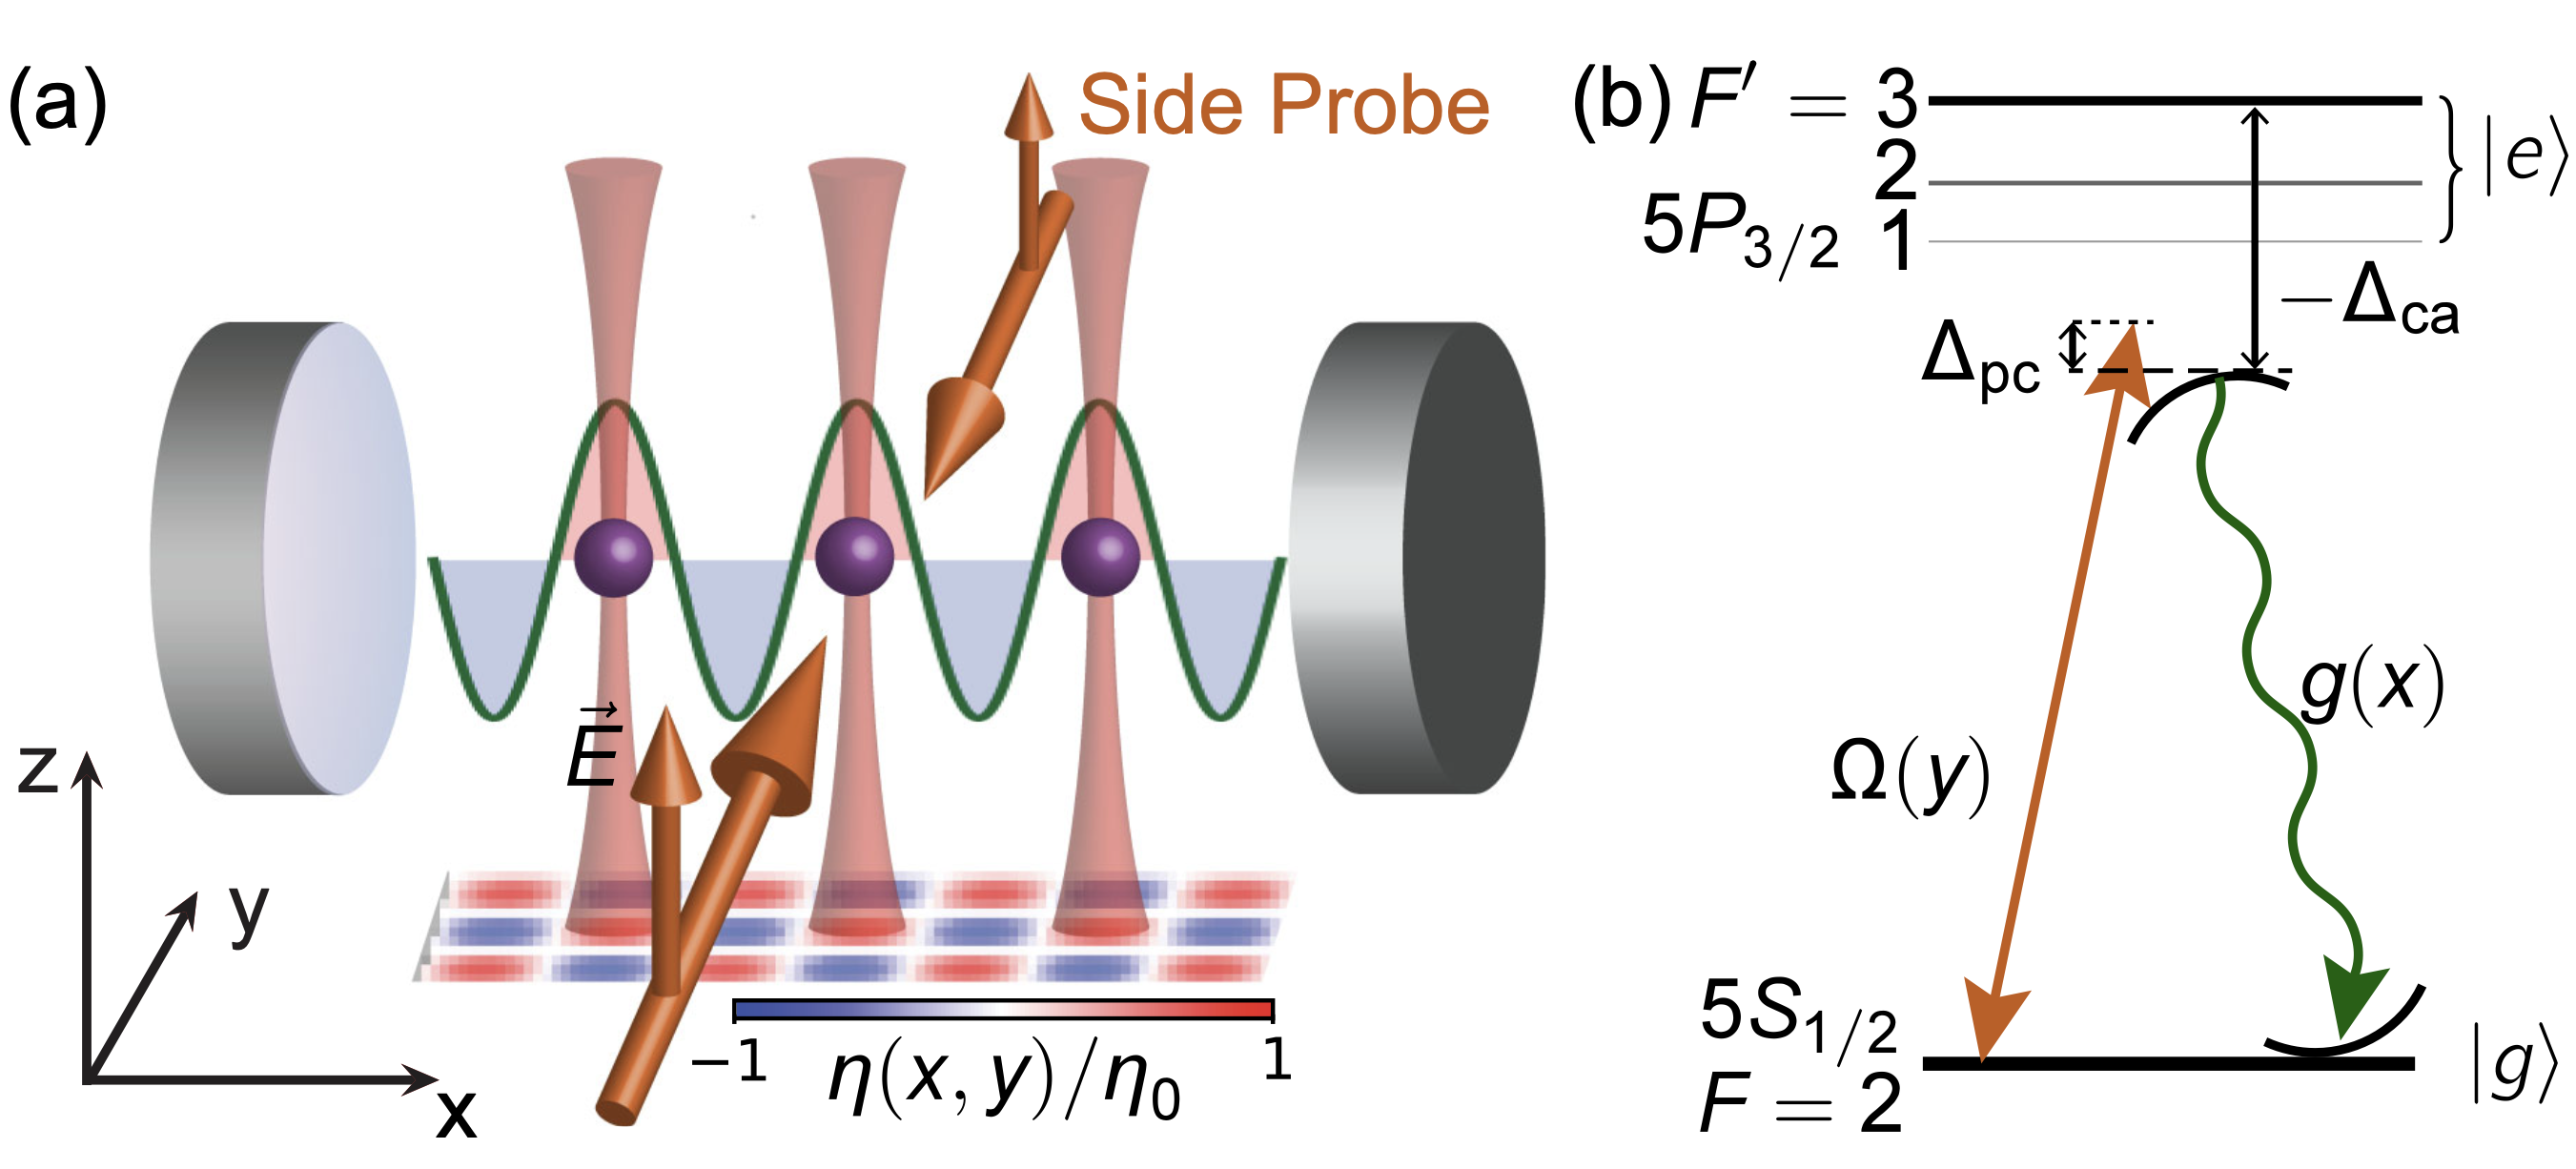
\includegraphics[width=0.8\textwidth]{Figure_1.png}
		\hspace{3em}
	\end{minipage}\newline
	\vspace{2em}
	\begin{minipage}{\textwidth}
		\begin{minipage}{0.57\textwidth}
			\begin{itemize}
				\item {\small 16 optical tweezers, $\sigma = 100\pm14\,$nm\pause}
				\item {\small cavity-atom coupling, $g(x)=g_0\cos(kx)$}\pause
				\item {\small laser-atom coupling, $\Omega(y)=\Omega_0\cos(ky)$}
			\end{itemize}
		\end{minipage}
		\begin{minipage}{0.42\textwidth}
			\centering
			$\,\lambda=780\,$nm\newline
			\alert{$\eta(x,y)=\eta_0\cos(kx)\cos(ky)$}
		\end{minipage}
	\end{minipage}
\end{frame}

\begin{frame}{Two-photons scattering}
	\begin{minipage}{0.4\textwidth}
		\centering
		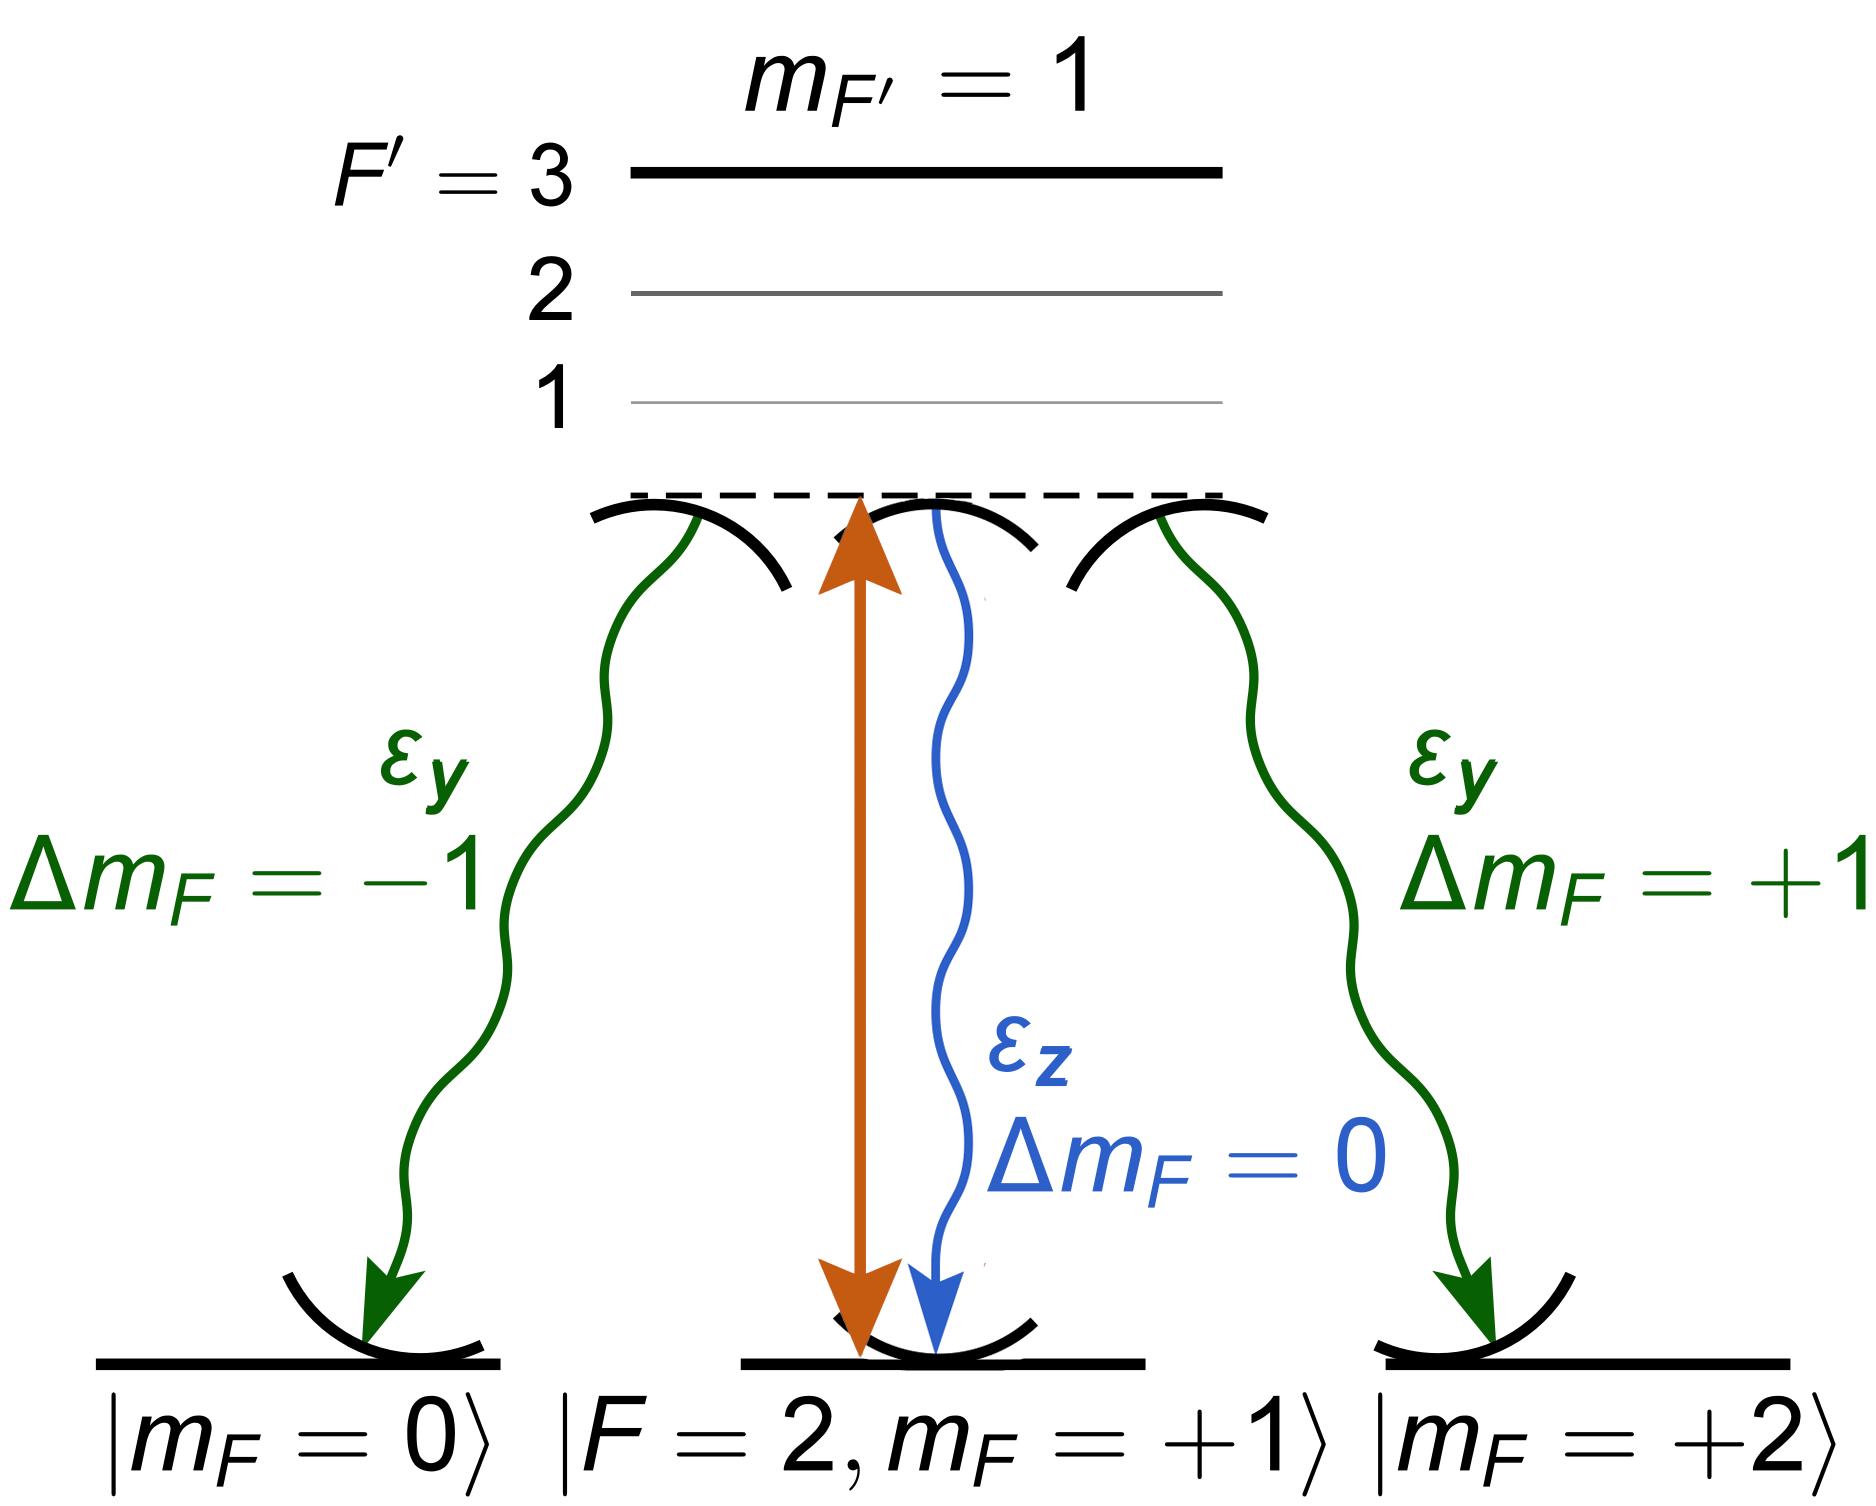
\includegraphics[width=\textwidth]{Figure_scattering_types.png}
	\end{minipage}
	\hfill
	\begin{minipage}{0.55\textwidth}
		\begin{center}
			Initial state: $\ket{m_{F,1},...,m_{F,i},...}\ket{0}_z\ket{0}_y$\pause
		\end{center}
		\vspace{2em}
		\textbf{Rayleigh scattering ($\Delta m_F=0$)}\\
		\vspace{-0.7em}
		\begin{equation*}
			\sum_{i=1}^N \eta^{Ray}_i\ket{m_{F,1},...,m_{F,i},...}\ket{1}_z\ket{0}_y\pause
		\end{equation*}\\~\\
		\textbf{Raman scattering ($\Delta m_F=\pm1$)}\\
		\vspace{-0.7em}
		\begin{equation*}
			\sum_{i=1}^N \eta^{Ram}_i\ket{m_{F,1},...,m_{F,i}\pm1,...}\ket{0}_z\ket{1}_y
		\end{equation*}
	\end{minipage}
\end{frame}

\begin{frame}{Two-photons scattering}
	In the dispersive coupling regime $|\Delta_{ca}|\gg\{\Omega_0,g_0,\gamma\}$, the cavity photon number, distinguished on the scattering process (thus on polarization), is
	\begin{align*}
		n^{Ray}_N &\propto |\sum_{i=1}^N \eta^{Ray}_i|^2\\
		n^{Ram}_N &\propto \sum_{i=1}^N |\eta^{Ram}_i|^2
	\end{align*}
\end{frame}

\begin{frame}{Real-experiment complications}
	\begin{itemize}
		\item Atoms are not perfectly localised
		\vspace{-1em}
		\begin{equation*}
			n^{Ray}_N \propto \int...\dd{x_i}\dd{y_i}... \rho(x_i,y_i)...\; |\sum_{i=1}^N \eta^{Ray}_i|^2
		\end{equation*}
		\item The Rayleigh scattering amplitude of the i-th atom reads
		\vspace{-1em}
		\begin{equation*}
			\eta^{Ray}_i = \sum_{F'=1}^3\eta^{Ray}_0(m_{F,i},F')\cos(kx_i)\cos(ky_i)
		\end{equation*}
	\end{itemize}
\end{frame}

\begin{frame}{Magic detuning}
	\begin{minipage}{\textwidth}
		\hspace{3em}
		\begin{minipage}{0.1\textwidth}
			\begin{align*}
				\text{At }\Delta_{ca}=-2\pi\times507\,\text{MHz}
			\end{align*}
		\end{minipage}
		\hspace{-1em}
		\begin{minipage}{0.49\textwidth}
			\begin{align*}
				&\longrightarrow \eta^{Ram}_i=0 \quad\forall i\\
				&\longrightarrow \eta^{Ray}_0(m_{F,i},F')=\eta^{Ray}_0(F')
				\end{align*}
		\end{minipage}
	\end{minipage}
	\vfill
	Also, the atom-induced modifications of the cavity resonance can be neglected for large $|\Delta_{ca}|$.
	\vfill
\end{frame}

\begin{frame}{Two atoms {\tiny at $y$=0 and magic detuning}}
	\begin{minipage}{\textwidth}
		\begin{minipage}{0.3\textwidth}
			\begin{equation*}
				n^{Ray}_N \propto |\sum_{i=1}^N \eta^{Ray}_i|^2
			\end{equation*}
			\vspace{1em}
			\begin{minipage}{\textwidth}
				\textbf{Ideal case}
				\vspace{-0.5em}
				\begin{equation*}
					\frac{n_2}{n_1} = \bigl(1+\cos(kd)\bigr)^2
				\end{equation*}
			\end{minipage}
			\vspace{0.8em}
		\end{minipage}
		\hfill
		\begin{minipage}{0.6\textwidth}
			\centering
			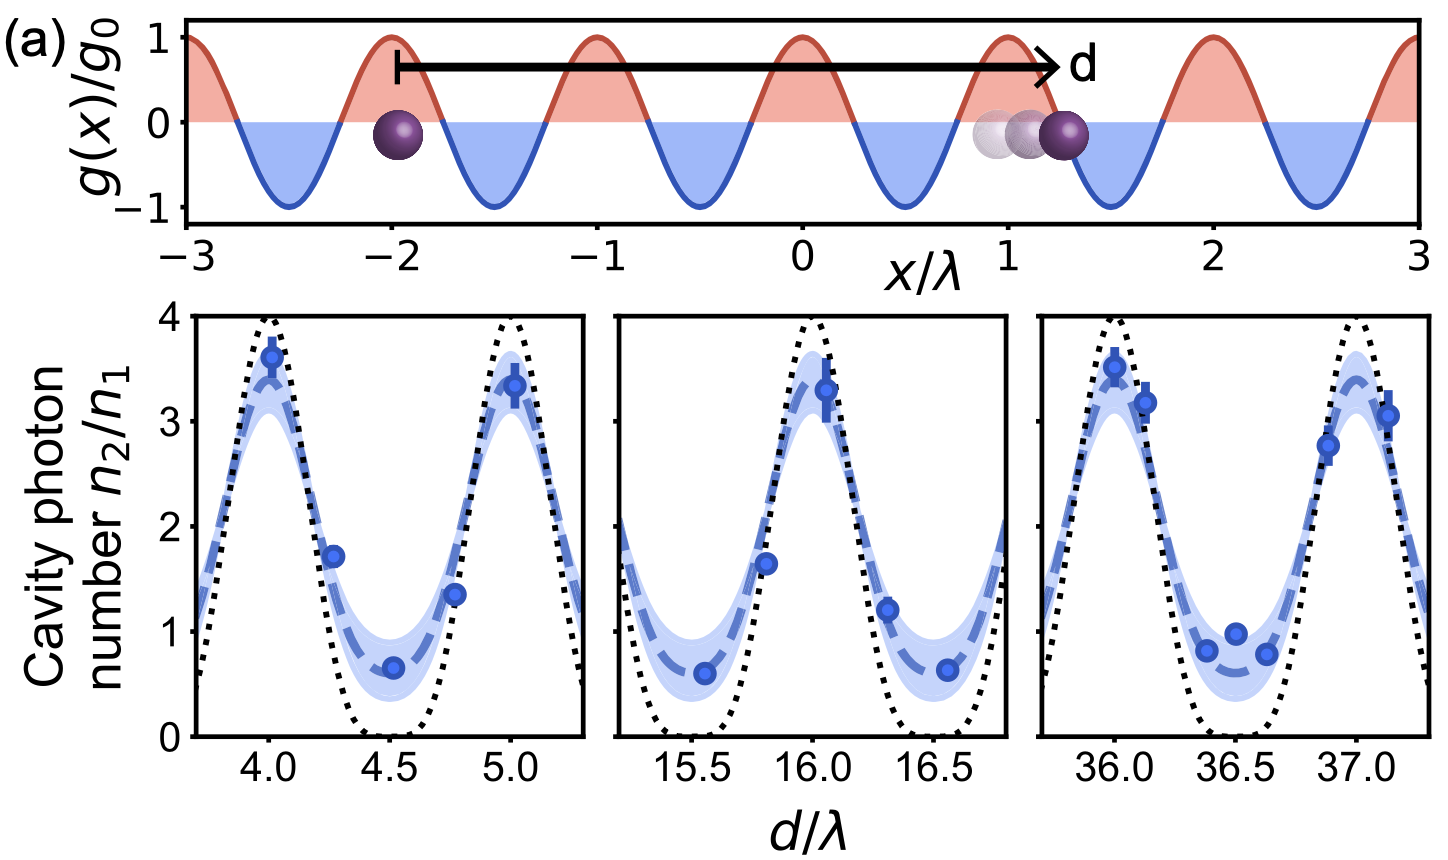
\includegraphics[width=\textwidth]{Figure_2a.png}
		\end{minipage}
	\end{minipage}\\
	\vfill
	\begin{minipage}{0.6\textwidth}		
		\textbf{Finite position fluctuations $\sigma$}
		\vspace{-0.5em}
		\begin{equation*}
			\frac{n_2}{n_1} = 1+\frac{C\cos(2kd)+1}{C+1}+8\frac{C\cos(kd)}{(C+1)^2}
		\end{equation*}
	\end{minipage}
	\hfill
	\begin{minipage}{0.35\textwidth}
		\vspace{1.4em}
		Cavity signal's contrast
		\vspace{-1em}
		\begin{equation*}
			C = e^{-k^2\sigma^2}
		\end{equation*}
	\end{minipage}
\end{frame}

\begin{frame}{More atoms {\tiny at $y$=0 and magic detuning}}
	\vspace{0.5em}
	\begin{minipage}{\textwidth}
		\centering
		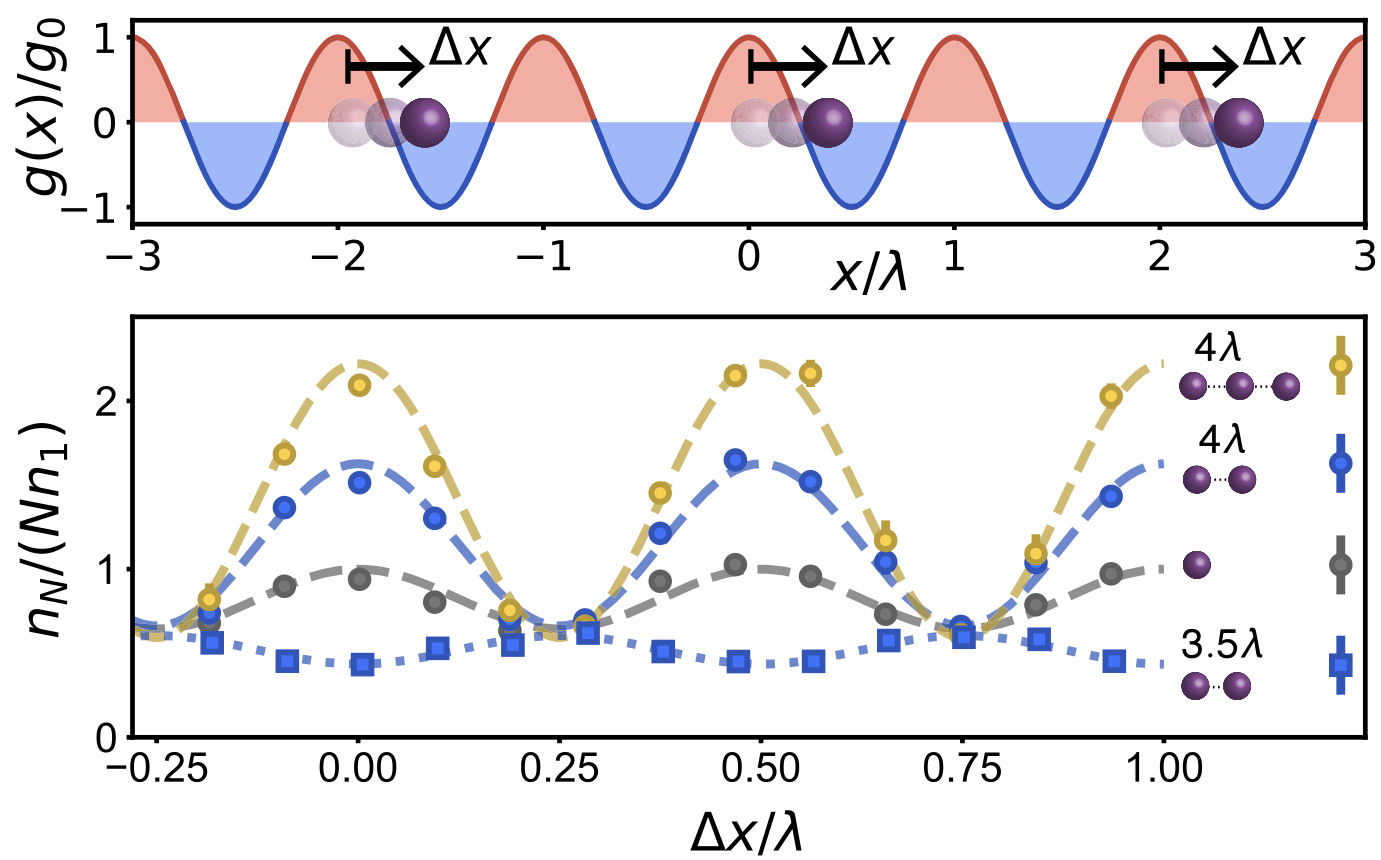
\includegraphics[width=0.6\textwidth]{Figure_2b.png}
	\end{minipage}
	{\small\begin{align*}
		\text{$\lambda$ spacing:}\quad \left(\frac{n_N}{N\;n_1}\right)_{max} &= \left(\frac{C-1}{C+1}\right)^2 + N\frac{4C}{(C+1)^2}\\
		\text{$\lambda/2$ spacing:}\,\quad \left(\frac{n_N}{N\;n_1}\right)_{min} &= \left(\frac{C-1}{C+1}\right)^2 + \frac{1}{N}\frac{4C}{(C+1)^2}\frac{1-(-1)^N}{2}
	\end{align*}}
\end{frame}

\begin{frame}{Scaling of $n_N$ with the atoms' number {\tiny at $y$=0}}
	\begin{minipage}{0.68\textwidth}
		\centering
		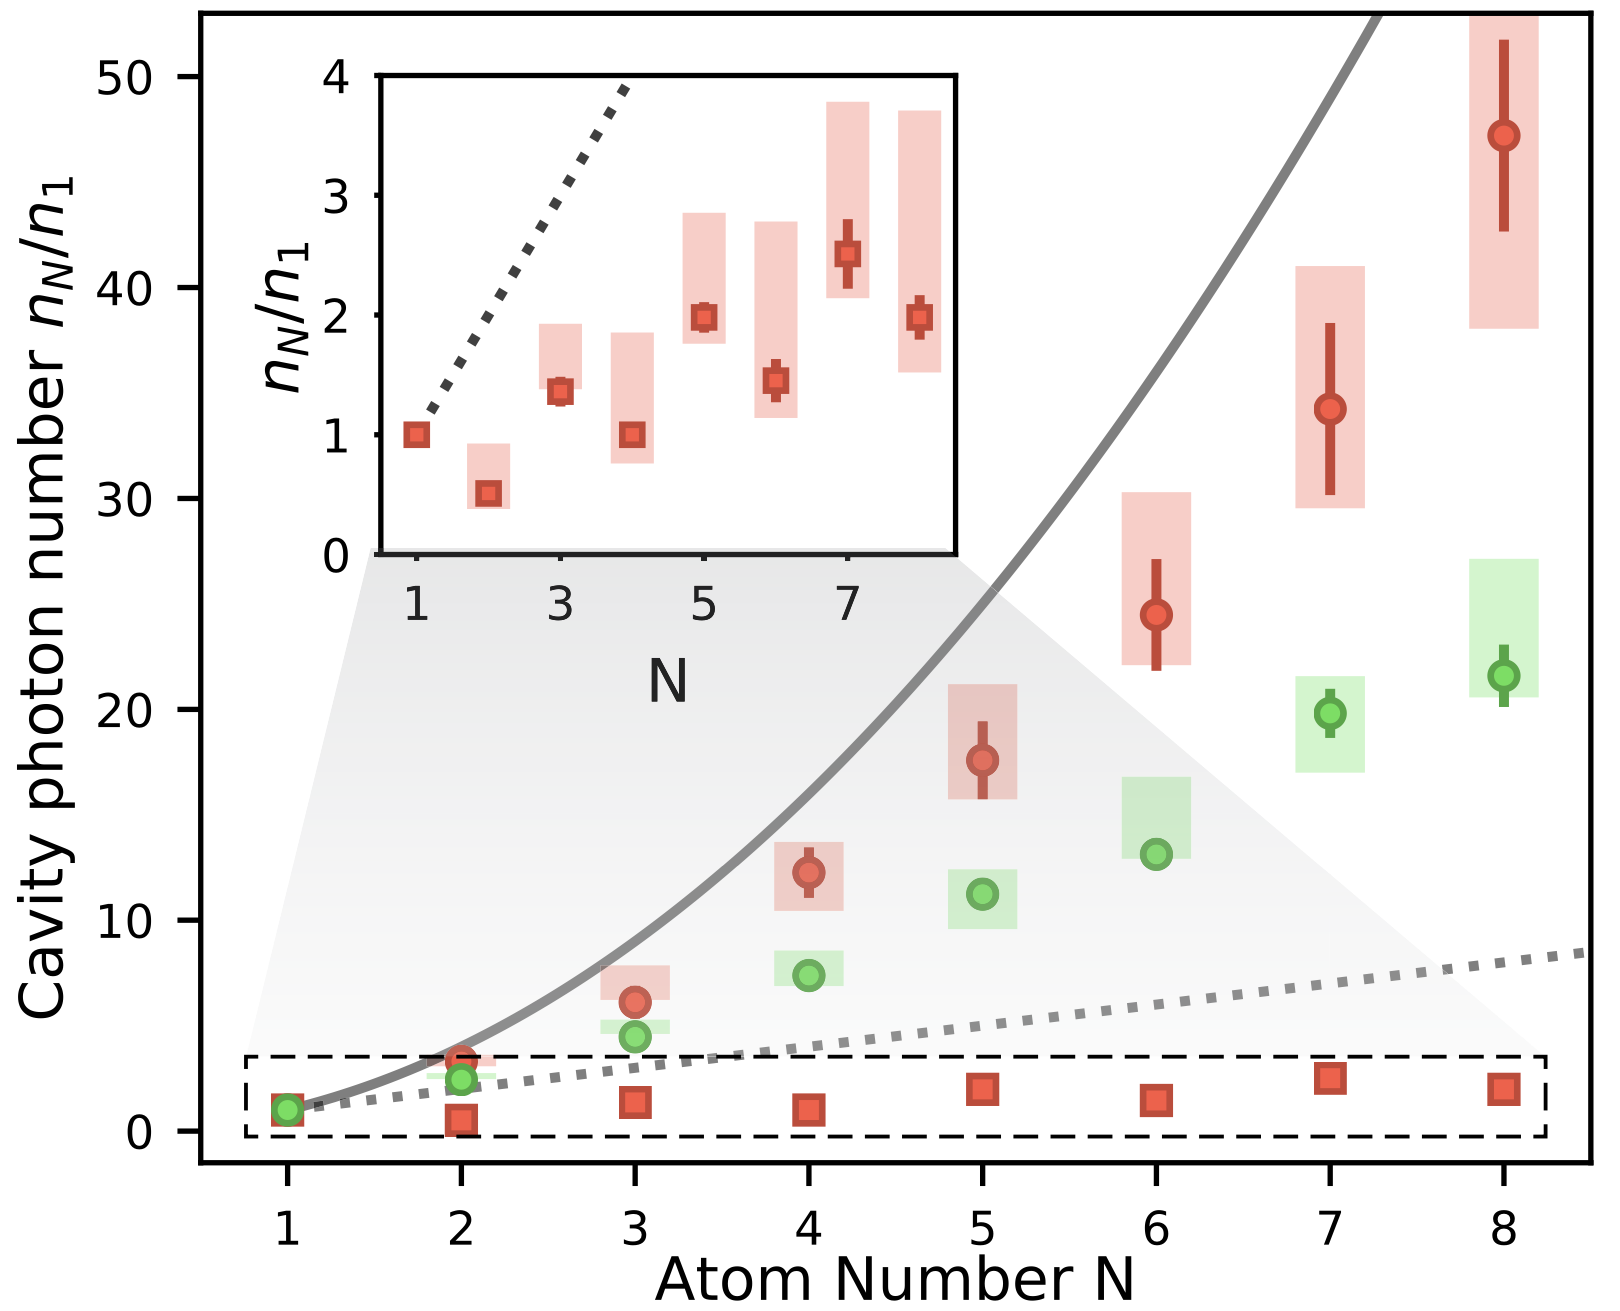
\includegraphics[width=\textwidth]{Figure_3a.png}
	\end{minipage}
	\begin{minipage}{0.31\textwidth}
		\textcolor[rgb]{0.859, 0.420, 0.329}{$\Delta_{ca}=-2\pi\times 507\,$MHz\\$\lambda$-spacing}\\
		\vspace{2.2em}
		\textcolor[rgb]{0.529, 0.851, 0.455}{\\$\Delta_{ca}=-2\pi\times 38\,$MHz\\$\lambda$-spacing}\\
		\vspace{2.5em}
		\textcolor[rgb]{0.859, 0.420, 0.329}{\\ $\Delta_{ca}=-2\pi\times 507\,$MHz\\$\lambda/2$-spacing}\\
	\end{minipage}
\end{frame}

\begin{frame}{Polarization analysis of the cavity emission {\tiny at $y$=0}}
	\begin{minipage}{0.49\textwidth}
		\centering
		$\quad\qquad\;\Delta_{ca}=-2\pi\times38\,$MHz\\~\\
		\vspace{-0.8em}
		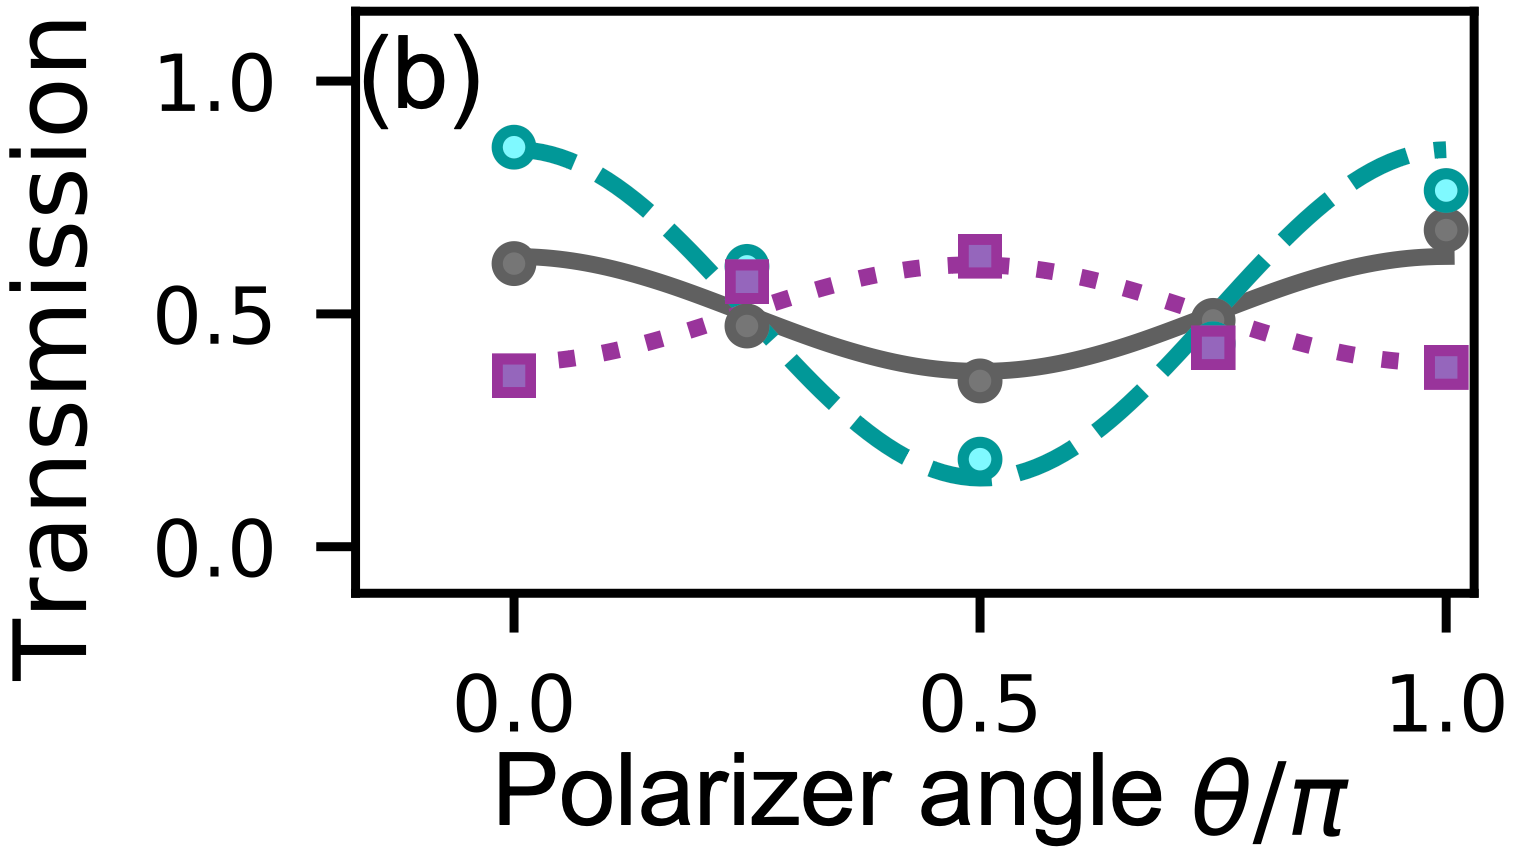
\includegraphics[width=\textwidth]{Figure_3b.png}
	\end{minipage}
	\hfill
	\begin{minipage}{0.49\textwidth}
		\centering
		$\;\;\Delta_{ca}=-2\pi\times507\,$MHz\\~\\
		\vspace{-0.8em}
		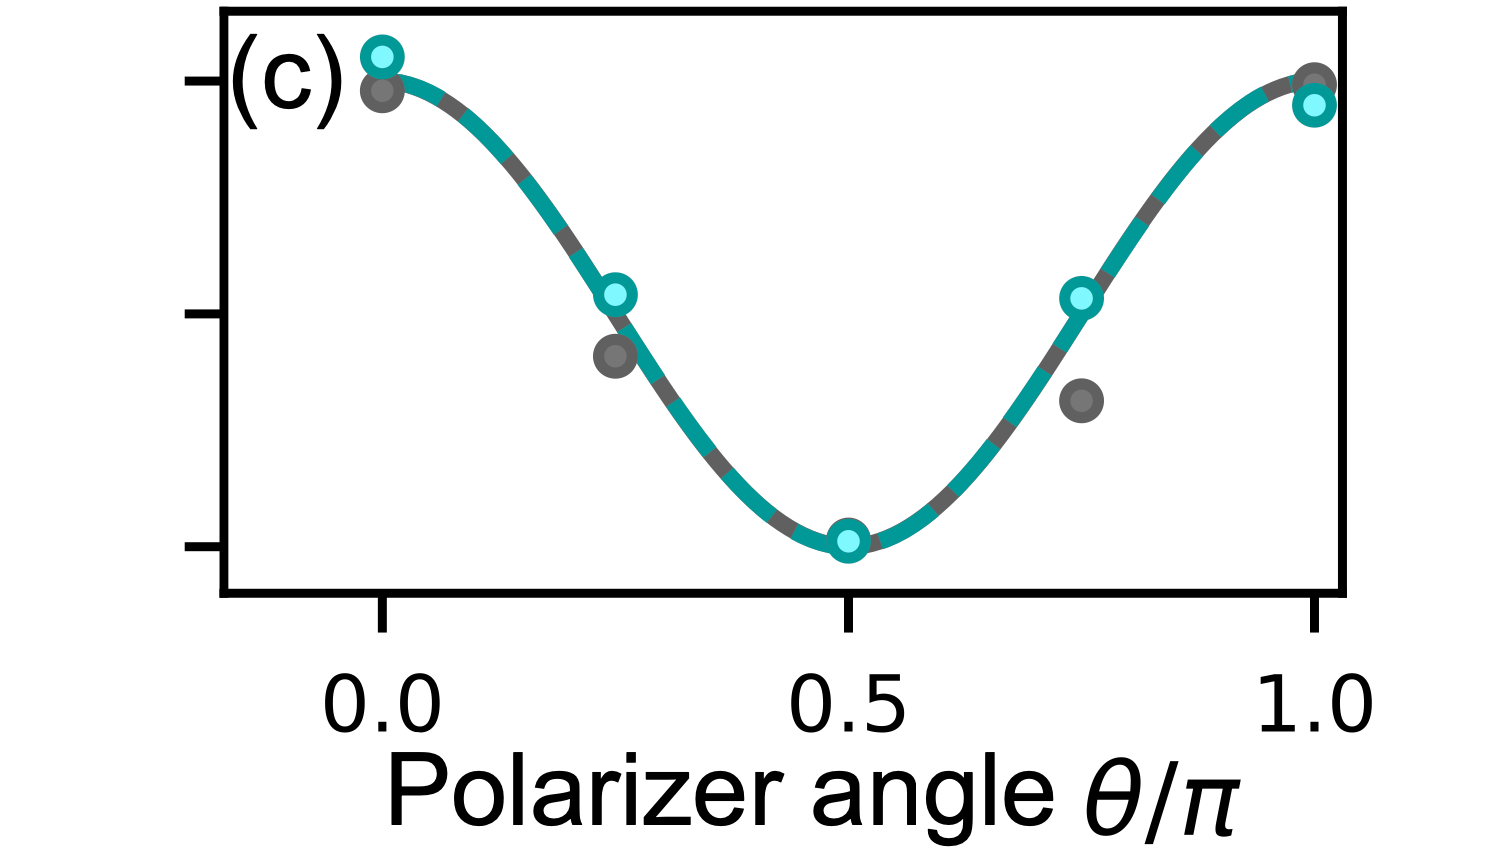
\includegraphics[width=\textwidth]{Figure_3c.png}
	\end{minipage}\\
	\vspace{2em}
	\begin{minipage}{0.2\textwidth}
		\vfill
		\begin{minipage}\textwidth
			Legend: $\begin{cases}
			~\\
			~\\
			~
			\end{cases}$
		\end{minipage}
		\vfill
	\end{minipage}
	\hspace{-2em}
	\begin{minipage}{0.33\textwidth}
		\textcolor[rgb]{0.376, 0.376, 0.376}{1 atom}\\
		\textcolor[rgb]{0.263, 0.588, 0.588}{8 atoms, $\lambda$-spacing}\\
		\textcolor[rgb]{0.553, 0.231, 0.376}{8 atoms, $\lambda/2$-spacing}
	\end{minipage}
	\hspace{-0.2em}
	\begin{minipage}{0.47\textwidth}
		{\footnotesize Using Raman scattered light ($\theta=\pi/2$) as a reference, integer-$\lambda$-spacing enhance Rayleigh scattering while half-integer-$\lambda$-spacing suppresses it.}
	\end{minipage}
\end{frame}

\begin{frame}{}
	\centering
	{\LARGE Thanks for your attention!}
\end{frame}

\begin{frame}{Atom-induced modifications of the cavity resonance}
	\begin{minipage}{0.38\textwidth}
		Atom-induced dispersive shift
		\begin{equation*}
			\sum_{i=1}^N \frac{g^2(x_i)}{\Delta_{ca}}
		\end{equation*}
		and absorptive broadening
		\begin{equation*}
			\sum_{i=1}^N\frac{\gamma g^2(x_i)}{\Delta^2_{ca}}
		\end{equation*}
	\end{minipage}
	\hfill
	\begin{minipage}{0.61\textwidth}
		\hspace{1.7em}
		\begin{minipage}{0.47\textwidth}
			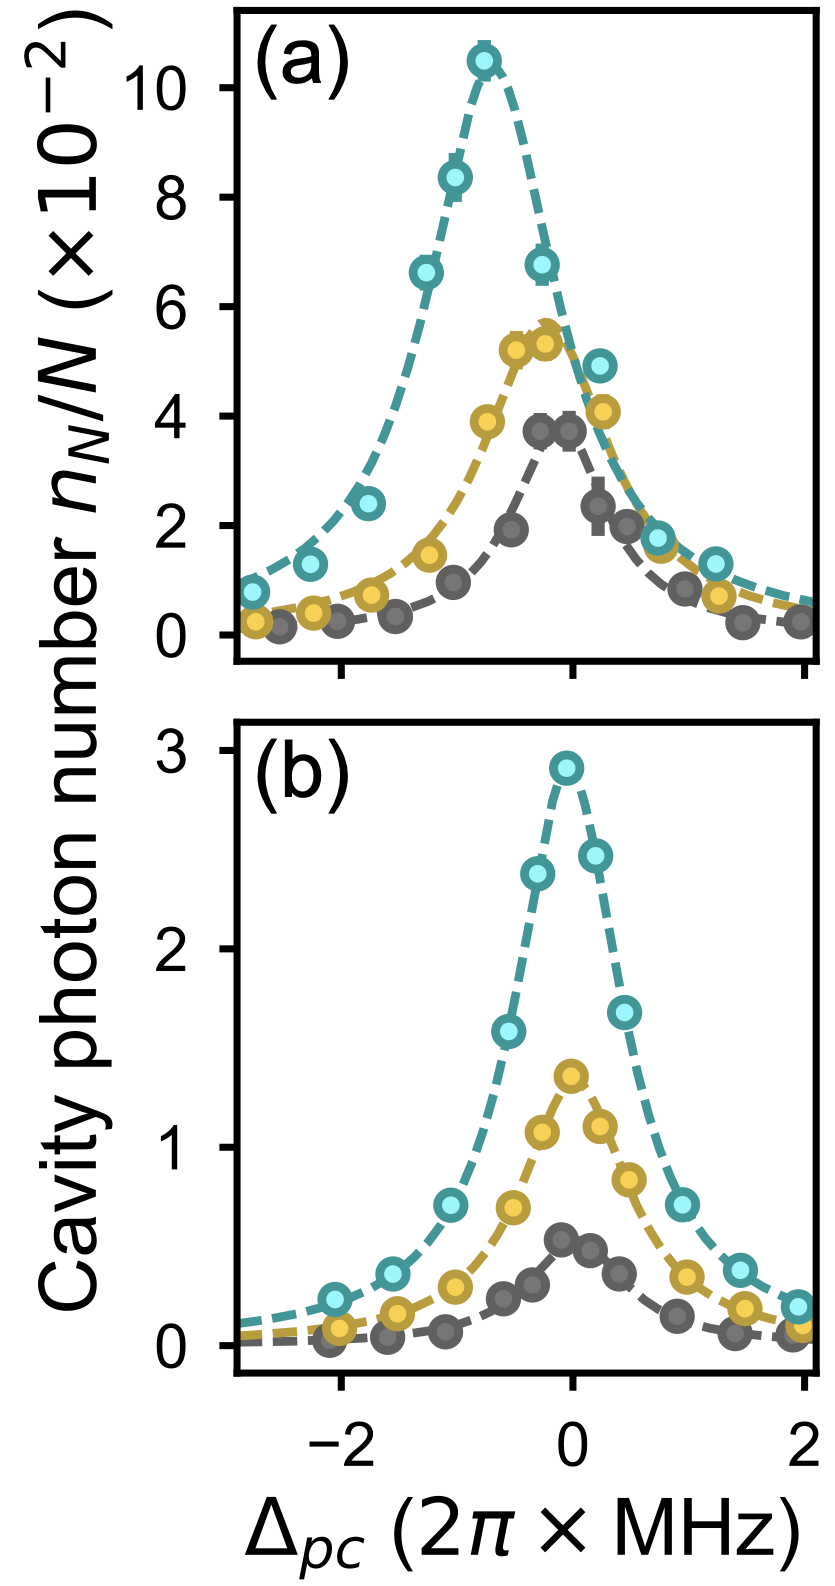
\includegraphics[width=0.9\textwidth]{Figure_4a.png}
		\end{minipage}
		\hspace{-1em}
		\begin{minipage}{0.42\textwidth}
			{\footnotesize$\Delta_{ca} = -2\pi\times38\,$MHz\\~\\
			\textcolor[rgb]{0.376, 0.376, 0.376}{~ ~1 atom}\\
			\textcolor[rgb]{0.725, 0.612, 0.243}{~ ~3 atoms, $\lambda$-spacing}\\
			\textcolor[rgb]{0.263, 0.588, 0.588}{~ ~8 atoms, $\lambda$-spacing}\\~\\
			\footnotesize$\Delta_{ca} = -2\pi\times507\,$MHz\\~}
		\end{minipage}
	\end{minipage}
\end{frame}

\begin{frame}{Atom-induced modifications of the cavity resonance}
	\begin{minipage}{0.5\textwidth}
		\centering
		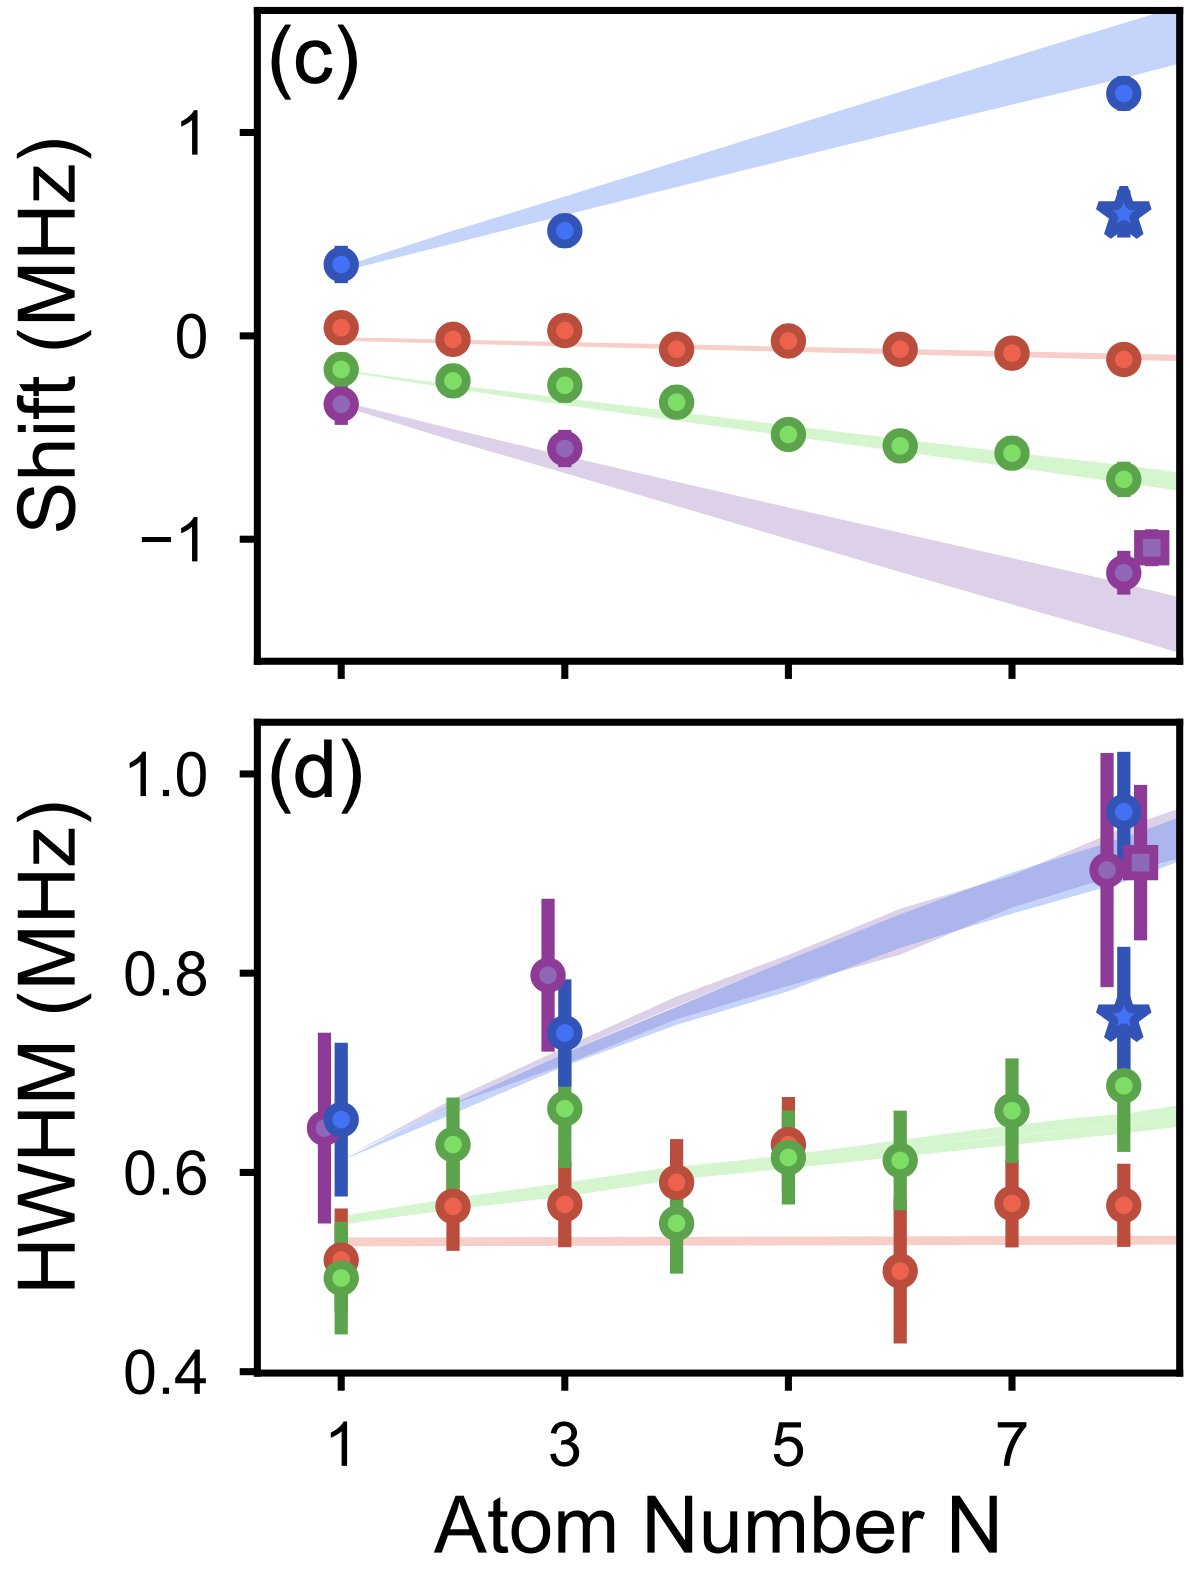
\includegraphics[width=0.8\textwidth]{Figure_4c.png}
	\end{minipage}
\end{frame}

\end{document}

